\section{Detailed Design}
\label{Section: design}


\begin{figure*}[!t]
	\centerline{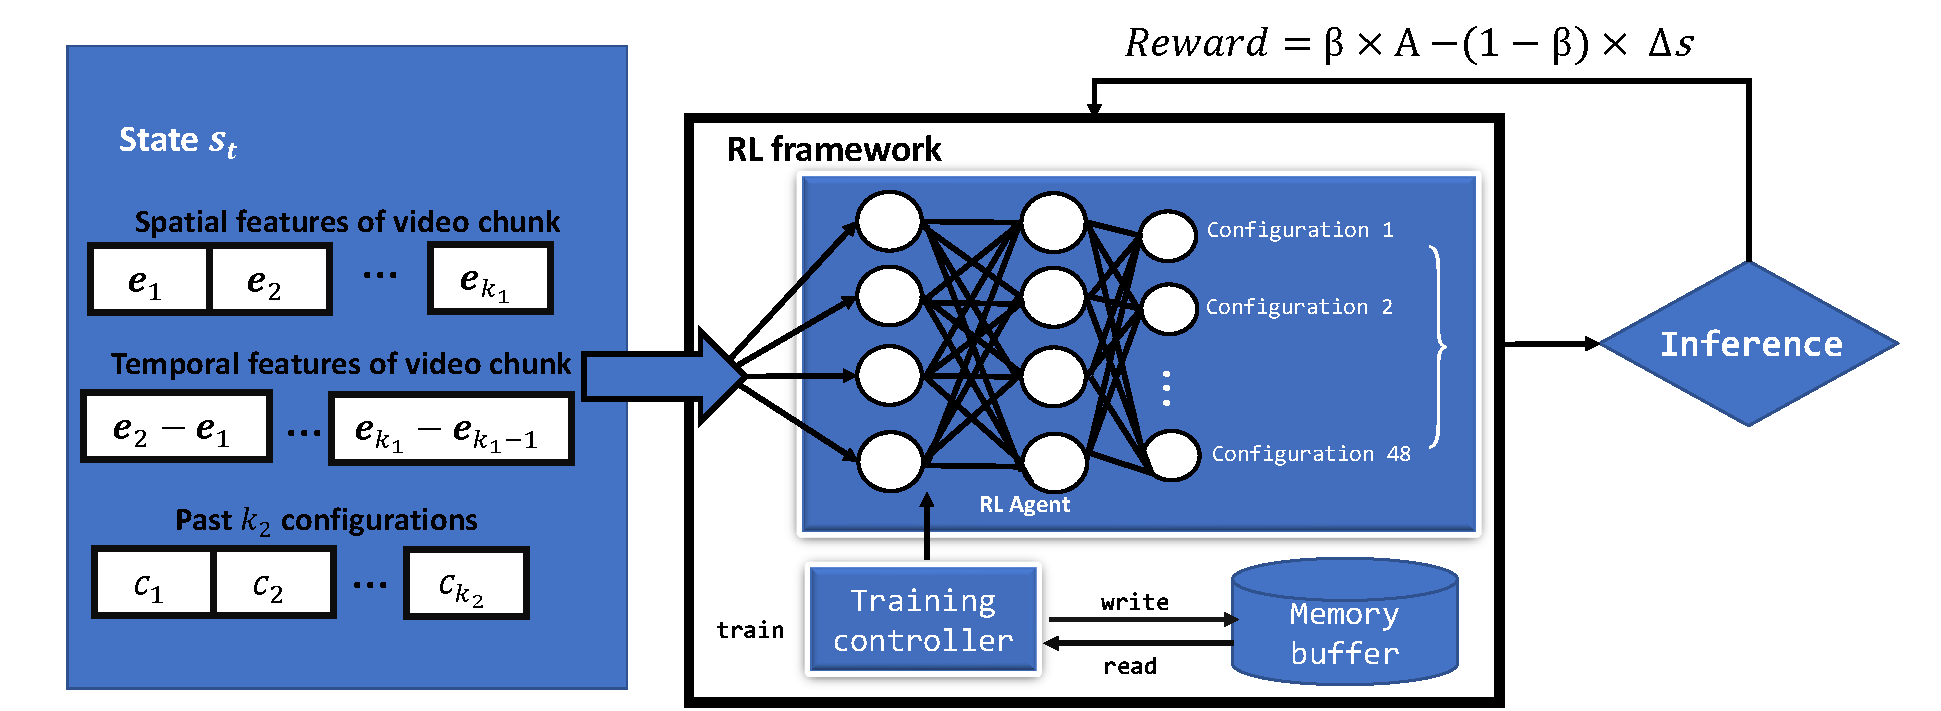
\includegraphics[width=0.9\linewidth]{figures/framework2.pdf}}
	%	\vspace{0.2cm}
	\caption{Applying reinforcement learning to automatic configuration}
	\label{fig: DQN}
\end{figure*}

Figure~\ref{fig: DQN} summarizes how RL can be applied to the automatic configuration. Briefly, it is a reinforcement learning-based system to train an agent to choose a proper configuration $ c $ for one video chunk to inference. We discuss the formulation, agent design, reinforcement learning-based framework, reward feedback in the following subsections. We provide experimental details of all the hyperparameters in Section~\ref{Section: experiment}. %% \\

\subsection{Problem Formulation}
\label{subsec: formulation}

To automaticly choose different configuration for video stream, we divides the video into T-second intervals as video chunks, and profiles configurations for each video chunk. Without loss of generality, we denote the object detection service as $ \vec{y}_i = M(x_i) $ that provides a predicted result list $ \vec{y}_i $ for each input video chunk $ x_i $. It has a baseline output $ \vec{y}_{\rm ref} = M(x_{\rm ref}) $ for each input video chunk $ x \in X_{\rm ref} $ using \emph{reference configuration} (the most expensive configuration). We use this $ \vec{y}_{\rm ref} $ as the ground truth label. For each video chunk $ x_c $ that uses a configuration $ c $, the output $ \vec{y}_c = M(x_c) $. Therefore, we have an accuracy metric $ \mathcal{A}_c $ by comparing $ \vec{y}_{\rm ref} $ and $ \vec{y}_c $. In general, we use the F1 score as the accuracy $ \mathcal{A} $, which is the harmonic mean of precision and recall, consistent with prior work~\cite{jiang2018chameleon,kang2017f1_noscope,zhang2017f1_live}. Besides, to compute the accuracy of a frame that was not sampled by $ c $, we use the location of objects from the previous sampled frame. 

For the cost of the object detection service, we use average GPU processing time per frame as the metric of resource consumption because GPU is the dominant resource for the majority of video processing workloads. We also denote the metric of resource consumption as $ \hat{s}_{ic} $ that for an input video chunk $ x_i $ and a given configuration $ c $. For a reference configuration $ c_{\rm ref} $, the reference resource consumption is $ \hat{s}_{\rm ref} $.

Initially, the agent tries different configurations $ c $ to obtain inference results image $ x_c $ from input video chunk $ x $. To obtain object detection results $ \{\vec{y}_{\rm ref}, \vec{y}_c\} $, the agent uses the choosen configuration $ c $ and the reference configuration $ x_{\rm ref} $. Comparing the two object detection results $ \{\vec{y}_{\rm ref}, \vec{y}_c\} $ and two resource consumptions $ \{\hat{s}_{\rm ref}, \hat{s}_c\} $, the agent computes the resource consumption ratio $ \Delta s = \frac{\hat{s}_c}{\hat{s}_{\rm ref}} $ and accuracy metric $ \mathcal{A}_c $.

\subsection{RL Agent Design}

The RL agent is expected to give a proper configuration $ c $ for minimizing the resource consumption $ \hat{s}_c $ while keeping the accuracy $ \mathcal{A} $. For the RL agent, the input features are continuous numerical vectors, and the expected output is discrete compression quality level $ c $. Therefore we can use the Deep Q-learning Network \cite{DQN} as the RL agent. But the naive Deep Q-learning Network can not work well in this task because the state space of reinforcement learning is too large if we directly treat video chunk as the input. To preserve enough details, we have to add many layers and nodes to the neural network, making the RL agent extremely difficult to converge.  
%because of the following challenges: %% \\
%
%\begin{itemize}
%	\item The state space of reinforcement learning is too large. To preserve enough details, we have to add many layers and nodes to the neural network, making the RL agent extremely difficult to converge. 
%	\item It takes a long time to train one step in a large inference neural network, making the training process too time-consuming.
%	\item The RL agent starts training from random trials and learns afterward from the reward feedback. When training from a randomly initialized neural network, the reward feedback is very sparse, making it difficult for the agent to learn.
%\end{itemize}

To address this challenges, we extract the top $k_1$ representative images from each chunk as spatial features of video chunk. We use a pre-trained small neural network to extract the structural information embeddings $ \{e_1,e_2,...,e_{k_1}\} $ of the images to reduce the input dimension and accelerate the training procedure. This is a commonly used strategy in training a deep neural network~\cite{finetunning,finetunning2}. In this work, we use the early convolution layers of MobileNetV2~\cite{MobileNetV2} as the image feature extractor $ \mathcal{E}(\cdot) $ for its efficiency in image classification. To extract the temporal features of video chunk, we obtain $ \{\hat{e}_1,\hat{e}_2,...,\hat{e}_{{k_1}-1}\} $ by each embedding subtracting previous embedding. Besides, we record the last $k_2$ configurations $ \{c_1,c_2,...,c_{k_2}\} $. To Solve that vectors of different lengths are not conducive to input to the neural network, we use fully connected layer to transform the spatial embedding $ \{e_1,e_2,...,e_{k_1}\} $, temporal embedding $ \{\hat{e}_1,\hat{e}_2,...,\hat{e}_{{k_1}-1}\} $, and recent configuration $ \{c_1,c_2,...,c_{k_2}\} $ to the fixed length vector, similar to the work~\cite{pensieve}. We formulate the fixed length vector $ s $ as \emph{states} and the configuration $ c $ as discrete \emph{actions}.

\subsection{Reinforcement Learning-based Framework}

In our system, we define 48 discrete actions to indicate 48 configuration, and the specific configurations are provided in Section~\ref{subsec: configuration}. We denote the \emph{action-value function} as $ Q(s, c; \theta) $ and the optimal compression quality level at time $ t $ as $  c_t = {\rm argmax}_cQ(s, c; \theta) $ where $ \theta $ indicates the parameters of the Deep Q-learning Network $ \phi $. In such reinforcement learning formulation, the training phase is to minimize the loss function $ L_i(\theta_i) = \mathbb{E}_{s, c \sim \rho (\cdot)}\Big[\big(y_i - Q(s, c; \theta_i)\big)^2 \Big] $ that changes at each iteration $ i $ where target $ y_i = \mathbb{E}_{s' \sim \{\mathcal{X}, M\}} \big[ r + \gamma \max_{c'} Q(s', c'; \theta_{i-1}) \mid s, c \big] $. Especially, $ r $ is the reward feedback, and $ \rho(s, c) $ is a probability distribution over state  $ s $ and the configuration $ c $~\cite{DQN}. When minimizing the distance of \emph{action-value function}'s output $ Q(\cdot) $ and target $ y_i $, the \emph{action-value function} $ Q(\cdot) $ outputs a more accurate estimation of an action. 

In the training phase, the RL agent firstly using an $\epsilon-$greedy method to take some random trials to observe the environment's reaction and decreases the randomness when training afterward. In iteration $t$, we input state $s_t $ to neural network $ \phi $. The RL agent $\phi$ generates a specific configuration $c_t$. The framework processes the video chunk $x_t$ using configuration $c_t$ to inference object detection services and obtains reward $r_t$. Then the framework obtains the next video chunk $x_{t+1}$ and generates the next state $ s_{t+1} $. The framework stores transition $(s_t, c_t, r_t, s_{t+1})$ in a memory buffer $\mathcal{D}$. Especially, the transition $(s_t, c_t, r_t, s_{t+1} )$ is uesd to compute the loss function. All transitions are saved into a memory buffer $ \mathcal{D} $, and the agent learns to optimize its \emph{action} by minimizing the loss function $ L $ on a mini-batch from $ \mathcal{D} $. The training procedure would converge when the agent's randomness keeps decaying. Finally, the agent's action is based on its historical ``optimal'' experiences. The training procedure is presented in Algorithm~\ref{alg: rl-train}.

\begin{algorithm}[!t]
		\caption{Training RL agent $ \phi $} %in environment $ \{\mathcal{X}, M\} $}
		\label{alg: rl-train}
		\begin{algorithmic}[1]	
			\STATE Initialize action-value function $ Q $ with random weights $ \theta $, replay memory buffer $ \mathcal{D} $ and state $ s_1 $				
			\FOR {$t \in 1,2,\cdots, K$}
			\STATE \textbf{1) Exploration}
			\STATE With probability $\epsilon$:
			\STATE \hspace{1em} $c_t \leftarrow$ a random valid value 
			\STATE Otherwise:
			\STATE \hspace{1em} $ c_t \leftarrow {\rm argmax}_cQ(s_t, c; \theta) $ 

			\STATE \textbf{2) Reward calcuation} 
			\STATE Process video chunk $ x_t $ using configuration $ c_t $ to inference
			\STATE Obtain $ (\vec{y}_{\rm ref}, \vec{y}_c) $ from the object detection service
			\STATE Compute reward $ r \leftarrow R(\Delta s, \mathcal{A}_c) $ according to \ref{subsec: reward} Reward Feedback Design 
			\STATE \textbf{3) Gradient descent}
			\STATE Obtain next video chunk $ x_{t+1} $
			\STATE Generate next state $ s_{t+1} $
			\STATE $ \mathcal{D} \leftarrow \mathcal{D} \bigcup \{(s_t, c_t, r_t, s_{t+1} \} $
			\STATE Sample a randomly mini-batch of transitions $ (s_j, c_j, r_j, s_{j+1}) $ from memory buffer $ \mathcal{D} $
			\STATE $ y_j \leftarrow r_j + \gamma \max_{c'}Q(s_{j+1}, c'; \theta) $
			\STATE Perform a gradient descent step on $ \big(y_j - Q(s_j, c_j; \theta)\big)^2 $ according to~\cite{DQN}
			\ENDFOR
		\end{algorithmic}
\end{algorithm}

\subsection{Reward Feedback Design}
\label{subsec: reward}

In our solution, the agent is trained by the reward feedback. In the above formulation, we define resource consumption rate $ \Delta s = \frac{\hat{s}_c}{\hat{s}_{\rm ref}} $ and accuracy metric $ \mathcal{A}_c $ at configuration $ c $. Basically, we want the agent to choose a proper configuration for minimizing the resource consumption while remaining acceptable accuracy. Therefore the overall reward $ r $ should be positively correlated with the accuracy $ \mathcal{A} $ while negatively with the resource consumption ratio $ \Delta s $. We introduce a balance factor $ \beta $ to form a linear combination $ r = \beta \mathcal{A} - (1-\beta) \Delta s  $ as the \emph{reward function} $ R(\Delta s, \mathcal{A}) $. %% \\
